\textbf{Chain Rule:}
$$\frac{dL}{dx} = \frac{dL}{dz}\frac{dz}{dx}$$ 
\begin{center}
    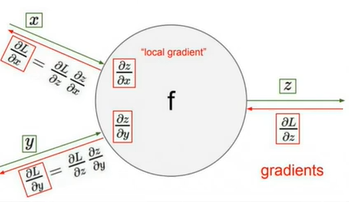
\includegraphics[]{22_1.PNG}
\end{center}
\textbf{BackPropagation} это метод вычисления градиента лосс-функции по параметрам\\

На картинке выше показан шаг BackPropagation для вычисления производной, причем сразу для векторных переменных.

На фазе forward-pass (когда вы пропускаете данные через сеть, умножая на матрицы и прочее), вычисляется выход
вершинки z, который определяется через какую-то функцию, затем вычисляются производные выхода по входам, т.е. $\frac{dz}{dx}$ и $\frac{dz}{dy}$, т.к. все данные для этого у нас есть.
После фазы forward pass’а начинается backward pass, где мы просто применяем Chain Rule на уже вычисленных
производных, вычисляя производные по всем параметрам.
\\

\textbf{Матричная форма}
\begin{center}
    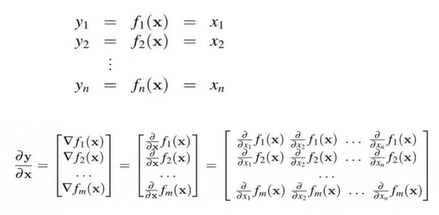
\includegraphics[scale=1.3]{22_3.PNG}
\end{center}

В этом-то умножении (chain rule) и состоит проблема затухания
градиента. Если ваш градиент станет очень маленьким в каком-то месте, то это просто не даст другим градиентам быть не
около 0, т.к. при умножении получается очень маленькое число. В этом случае gradient flow прекращается и сеть перестает
учиться. 
